\documentclass[a4paper,12pt]{report}
\usepackage[utf8]{inputenc}
\usepackage[T1]{fontenc}
\usepackage[french]{babel}
\usepackage{graphicx} % pour inclure des images
\usepackage{geometry}
\usepackage{listings} % pour le code source
\usepackage{amsmath} % pour les équations mathématiques
\usepackage{fancyhdr} % pour les en-têtes et pieds de page
\usepackage{url} % pour les liens URL
\usepackage{xcolor} % pour changer la couleur du texte

\geometry{hmargin=2.5cm,vmargin=3cm} % marges

\title{
    \textbf{ISIMA - Deuxième Année}\\
    \vspace{1cm}
    \Huge Laboratoire \#2 : Génération de Variates Aléatoires
}

\author{
    \textbf{Nom : Benkhali}\\
    Groupe : ISIMA \\
    Professeur : Dr. David Hill \\
    Date : \today
}

\date{}

% Configuration des en-têtes et pieds de page
\pagestyle{fancy}
\fancyhf{} % Efface les en-têtes et pieds de page par défaut
\fancyfoot[L]{Benkhali Khalil} % Nom en bas à gauche
\fancyfoot[R]{\thepage} % Numéro de page en bas à droite

\begin{document}

\maketitle % Crée la page de titre

\newpage

% Table des matières
\tableofcontents

\newpage

\chapter*{Introduction} % Introduction sans numéro de chapitre
\addcontentsline{toc}{chapter}{Introduction} % Ajoute l'introduction à la table des matières
Ce rapport présente la génération de variates aléatoires en utilisant le générateur Mersenne Twister. Les différentes méthodes de génération, y compris les distributions uniformes, exponentielles et discrètes, ainsi que la méthode de Box-Muller pour les lois normales, sont explorées.

\newpage
\section*{Partie 1 : Implémentation du Mersenne Twister}
\addcontentsline{toc}{section}{Partie 1 : Implémentation du Mersenne Twister} % Ajoute Partie 1 à la table des matières

\subsection*{Recherche et Téléchargement}
\addcontentsline{toc}{subsection}{Recherche et Téléchargement} % Ajoute Recherche et Téléchargement à la table des matières
Nous avons trouvé l'implémentation C du Mersenne Twister sur la page de Matsumoto. Le code source a été téléchargé et décompressé à l'aide de la commande suivante :

\begin{lstlisting}[language=bash]
tar zxvf mt19937-2002.tgz
\end{lstlisting}

\subsection*{Compilation et Test}
\addcontentsline{toc}{subsection}{Compilation et Test} % Ajoute Compilation et Test à la table des matières
Pour compiler l'implémentation, nous avons utilisé :

\begin{lstlisting}[language=bash]
gcc mt19937-2002.c -o mt_test
\end{lstlisting}

Après compilation, nous avons exécuté le programme pour vérifier la reproductibilité des résultats, en utilisant les fonctions \texttt{genrand\_int32} et \texttt{genrand\_real1}. Voici un exemple de code de test :

\begin{lstlisting}[language=C]
#include "mt19937ar.h"
#include <stdio.h>

int main() {
    init_genrand(5489); // Initialisation du générateur avec une graine
    printf("10 nombres pseudo-aléatoires générés :\n");
    for (int i = 0; i < 10; i++) {
        printf("genrand_int32: %u, genrand_real1: %f\n", genrand_int32(), genrand_real1());
    }
    return 0;
}
\end{lstlisting}

\subsection*{Commentaires}
\addcontentsline{toc}{subsection}{Commentaires} % Ajoute Commentaires à la table des matières
Les sorties obtenues étaient conformes aux résultats attendus, confirmant la bonne implémentation du générateur Mersenne Twister.

\newpage
\section*{Partie 2 : Génération de Nombres Uniformes}
\addcontentsline{toc}{section}{Partie 2 : Génération de Nombres Uniformes} % Ajoute Partie 2 à la table des matières

\subsection*{But de la Partie}
\addcontentsline{toc}{subsection}{But de la Partie} % Ajoute But de la Partie à la table des matières
Nous allons générer des nombres uniformes entre \([-98, 57.7]\) à l'aide de la fonction `uniform`.

\subsection*{Implémentation}
\addcontentsline{toc}{subsection}{Implémentation} % Ajoute Implémentation à la table des matières
La fonction `uniform` est définie comme suit :

\begin{lstlisting}[language=C]
double uniform(double a, double b) {
    return a + (b - a) * genrand_real1();
}
\end{lstlisting}

\subsection*{Résultats}
\addcontentsline{toc}{subsection}{Résultats} % Ajoute Résultats à la table des matières
Voici quelques exemples de nombres générés :

\begin{itemize}
    \item -59.30, -63.35, 50.89, 55.31, -89.75
\end{itemize}

\subsection*{Visualisation}
\addcontentsline{toc}{subsection}{Visualisation} % Ajoute Visualisation à la table des matières
L'histogramme montrant la répartition des nombres générés est affiché ci-dessous :

\begin{figure}[h!]
    \centering
    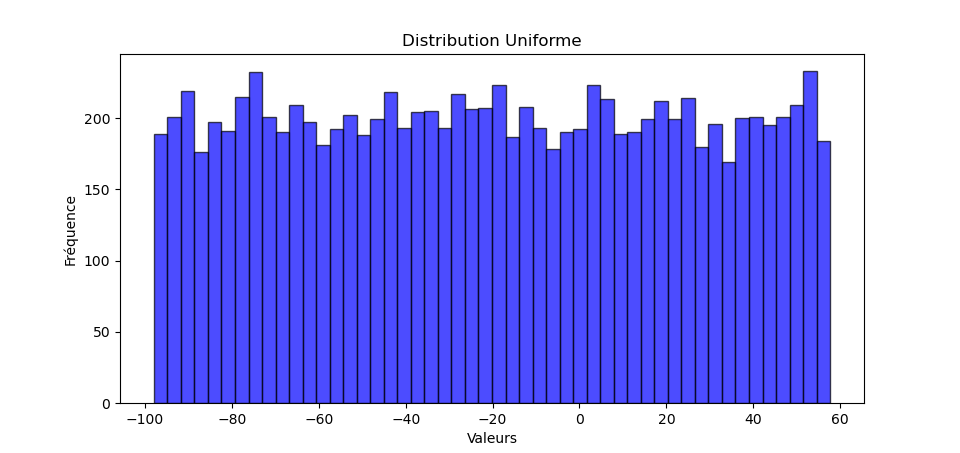
\includegraphics[width=0.8\textwidth]{1.png}
    \caption{Distribution uniforme des nombres entre -98 et 57.7}
\end{figure}

\subsection*{Commentaires}
\addcontentsline{toc}{subsection}{Commentaires} % Ajoute Commentaires à la table des matières
L'histogramme montre une distribution uniforme, ce qui valide le bon fonctionnement de la fonction `uniform`.

\newpage
\section*{Partie 3 : Reproduction de Distributions Empiriques Discrètes}
\addcontentsline{toc}{section}{Partie 3 : Reproduction de Distributions Empiriques Discrètes} % Ajoute Partie 3 à la table des matières

\subsection*{But de la Partie}
\addcontentsline{toc}{subsection}{But de la Partie} % Ajoute But de la Partie à la table des matières
Nous allons simuler une distribution discrète avec trois classes : A, B et C. Les proportions respectives de ces classes sont 35\%, 45\%, et 20\%.

\subsection*{Implémentation}
\addcontentsline{toc}{subsection}{Implémentation} % Ajoute Implémentation à la table des matières
Nous avons implémenté la simulation comme suit :

\begin{lstlisting}[language=C]
void simulate_discrete(int n) {
    int countA = 0, countB = 0, countC = 0;

    for (int i = 0; i < n; i++) {
        double r = genrand_real1();
        if (r < 0.35) countA++;
        else if (r < 0.80) countB++;
        else countC++;
    }

    printf("Classe A: %.2f%%\n", (double)countA / n * 100);
    printf("Classe B: %.2f%%\n", (double)countB / n * 100);
    printf("Classe C: %.2f%%\n", (double)countC / n * 100);
}
\end{lstlisting}

\subsection*{Résultats}
\addcontentsline{toc}{subsection}{Résultats} % Ajoute Résultats à la table des matières
Les résultats de la simulation pour différents nombres d'échantillons sont :

\begin{itemize}
    \item 1 000 échantillons : Classe A: 34.20\%, Classe B: 45.50\%, Classe C: 20.30\%
    \item 10 000 échantillons : Classe A: 35.47\%, Classe B: 44.45\%, Classe C: 20.08\%
    \item 100 000 échantillons : Classe A: 34.93\%, Classe B: 45.04\%, Classe C: 20.03\%
    \item 1 000 000 échantillons : Classe A: 35.03\%, Classe B: 44.96\%, Classe C: 20.01\%
\end{itemize}

\subsection*{Visualisation}
\addcontentsline{toc}{subsection}{Visualisation} % Ajoute Visualisation à la table des matières
L'histogramme ci-dessous illustre la répartition des classes :

\begin{figure}[h!]
    \centering
    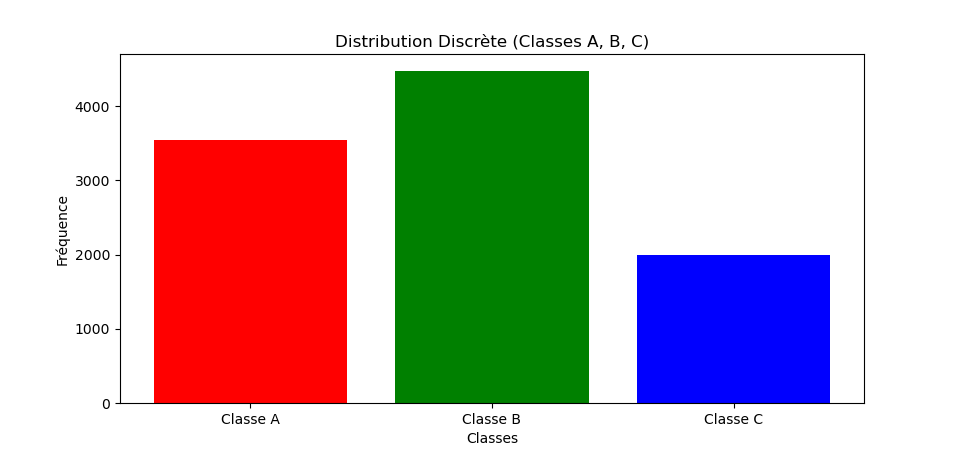
\includegraphics[width=0.8\textwidth]{3.png}
    \caption{Distribution discrète des classes A, B et C}
\end{figure}

\subsection*{Commentaires}
\addcontentsline{toc}{subsection}{Commentaires} % Ajoute Commentaires à la table des matières
Les résultats sont conformes aux attentes, montrant que la simulation est correcte.

\newpage
\section*{Partie 4 : Reproduction de Distributions Continues}
\addcontentsline{toc}{section}{Partie 4 : Reproduction de Distributions Continues} % Ajoute Partie 4 à la table des matières

\subsection*{But de la Partie}
\addcontentsline{toc}{subsection}{But de la Partie} % Ajoute But de la Partie à la table des matières
Nous allons reproduire une distribution continue en utilisant une loi exponentielle négative et la méthode d'inversion.

\subsection*{Implémentation}
\addcontentsline{toc}{subsection}{Implémentation} % Ajoute Implémentation à la table des matières
La fonction `negExp` est définie comme suit :

\begin{lstlisting}[language=C]
double negExp(double mean) {
    double random_number = genrand_real1();
    return -mean * log(1 - random_number);
}
\end{lstlisting}

\subsection*{Visualisation}
\addcontentsline{toc}{subsection}{Visualisation} % Ajoute Visualisation à la table des matières
L'histogramme ci-dessous montre la répartition des 10 000 nombres générés suivant la loi exponentielle négative :

\begin{figure}[h!]
    \centering
    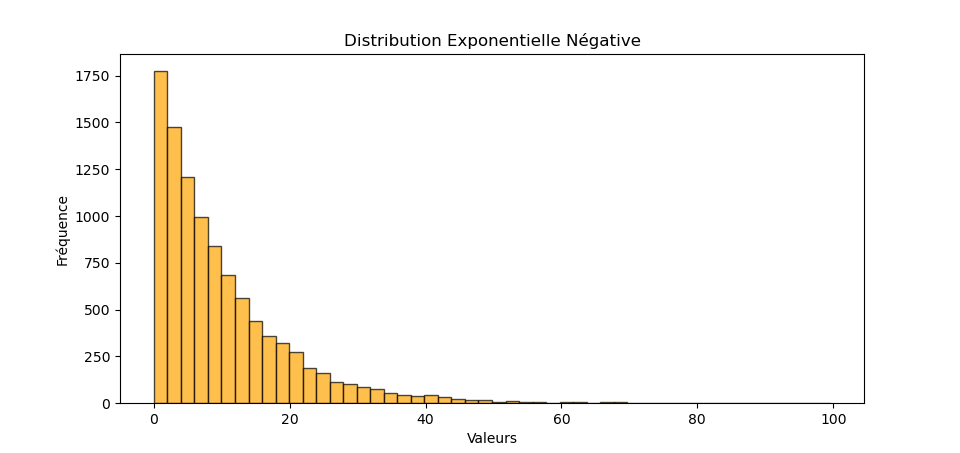
\includegraphics[width=0.8\textwidth]{2.png}
    \caption{Distribution exponentielle négative des nombres générés}
\end{figure}

\subsection*{Commentaires}
\addcontentsline{toc}{subsection}{Commentaires} % Ajoute Commentaires à la table des matières
La distribution générée montre que la plupart des nombres sont concentrés autour de petites valeurs, ce qui est typique d'une loi exponentielle négative.

\newpage
\section*{Partie 5 : Simulation de Lois Non-Réversibles}
\addcontentsline{toc}{section}{Partie 5 : Simulation de Lois Non-Réversibles} % Ajoute Partie 5 à la table des matières

\subsection*{But de la Partie}
\addcontentsline{toc}{subsection}{But de la Partie} % Ajoute But de la Partie à la table des matières
Nous allons utiliser la méthode de rejet pour générer des nombres selon une loi normale.

\subsection*{Implémentation}
\addcontentsline{toc}{subsection}{Implémentation} % Ajoute Implémentation à la table des matières
La méthode de Box-Muller est utilisée pour générer des nombres suivant une loi normale.

\subsection*{Visualisation}
\addcontentsline{toc}{subsection}{Visualisation} % Ajoute Visualisation à la table des matières
L'histogramme ci-dessous montre la répartition des nombres générés par la méthode de Box-Muller :

\begin{figure}[h!]
    \centering
    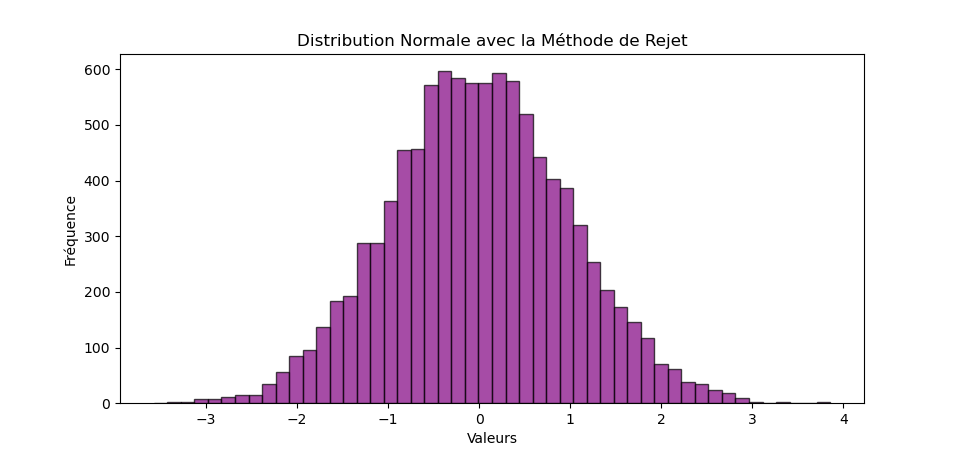
\includegraphics[width=0.8\textwidth]{4.png}
    \caption{Distribution normale générée par la méthode de Box-Muller}
\end{figure}

\subsection*{Commentaires}
\addcontentsline{toc}{subsection}{Commentaires} % Ajoute Commentaires à la table des matières
La courbe obtenue est symétrique autour de zéro, ce qui confirme l'efficacité de la méthode de Box-Muller pour générer des nombres suivant une distribution normale.

\newpage
\chapter*{Ouverture sur la Théorie de la Percolation}
\addcontentsline{toc}{chapter}{Ouverture sur la Théorie de la Percolation} % Ajoute l'ouverture à la table des matières
Dans le cadre de ce laboratoire, il est intéressant de faire un lien entre les techniques de génération de nombres aléatoires et la théorie de la percolation. En effet, la percolation est une branche des mathématiques qui étudie le comportement des réseaux et des milieux désordonnés. La génération de réseaux aléatoires, par exemple, repose sur des algorithmes de génération de nombres aléatoires, permettant de simuler des phénomènes tels que la propagation d'infections ou la diffusion de fluides.

L'utilisation de générateurs de haute qualité, comme le Mersenne Twister, est cruciale pour obtenir des simulations précises et fiables. En appliquant ces techniques à des modèles de percolation, nous pouvons explorer des comportements critiques dans des systèmes complexes, mettant en lumière l'importance de la génération de nombres aléatoires dans des contextes variés.

\newpage
\chapter*{Références}
\addcontentsline{toc}{chapter}{Références} % Ajoute la section Références à la table des matières

\begin{itemize}
    \item [1] D. D. Hill, “Lab 2 : Generation of random variates,” \url{https://perso.isima.fr/dahill/}, p. 2.
    \item [2] Code source disponible à l'adresse suivante : \url{https://github.com/Khalil9528/random_number.git}
\end{itemize}

\end{document}
